\newpage


\section{Reproductive plan}\label{sec:reproductive-plan}

This section describes a reproductive plan used in this thesis
– a process that takes a population on input and produces a modified population using genetic operators.
The reproductive plan has two main properties that have to be well-balanced with respect to each other
– diversification and intensification~\cite{blumMetaheuristicsCombinatorialOptimization2003}.\\

\navesti{Intensification} is the ability to identify parts of the search space with a high-quality
solutions.\\

\navesti{Diversification} is the ability to prevent premature convergence to the suboptimal solutions.\\

We can classify operators in terms of their intensification and diversification effects.
The mutation operator is considered to be the most straightforward diversification strategy,
as it creates a small change in an individual's chromosome that can lead the search out of the suboptimal solution~\cite{blumMetaheuristicsCombinatorialOptimization2003}.
On the other hand, crossover creates a new solution by recombination of already present
individuals, which can be considered diversification strategy~\cite{blumMetaheuristicsCombinatorialOptimization2003}.
However, researchers in~\cite{hanshengBalanceExplorationExploitation1999} argue that crossover
also has an intensification effect. They make an argument that if the population was primarily composed of the same individuals, the crossover would not be able to improve the solution.

\subsection{Strategy}\label{subsec:strategy}
The strategy for a reproductive plan used in this thesis is in figure~\ref{fig:population-schema}.
It has two parts – generating the initial population and transitioning from one generation to the next.
After each application of the reproductive plan, the number of individuals is the same.
This means that population size is a fixed hyperparameter of the genetic approach.

\begin{figure}[!htp]
    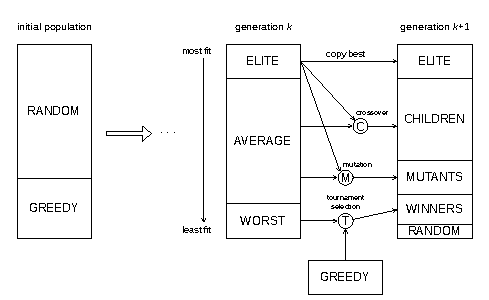
\includegraphics[width=0.8\textwidth, left]{pupulation_schema}\caption{Initial population generation strategy and transition from generation $k$ to $k+1$.}
    \label{fig:population-schema}
\end{figure}

\subsubsection*{Initial population}
The initial population is the population that is used as a starting point for the genetic approach.
It consists of two parts – RANDOM and GREEDY. \\

\navesti{RANDOM} part consists of randomly generated individuals.
The process of generating is (1) fill all two vectors and matrix of an individual chromosome with random values from $\langle 0,1 \rangle$
and then (2) normalize to stochastic vectors to meet constraints in~\ref{eq:constraints}.\\

\navesti{GREEDY} part consists of individuals who are, at worst, as good as RANDOM.
The process of generating $k$ GREEDY individuals is (1) to create $100k$ RANDOM individuals and (2) to select $k$ best ones
in terms of their objective value.\\

\todo{zminit duvod, proc je to zrovna takhle}

\subsubsection*{Population transition}
After generating the initial population, the genetic approach transforms the current population
to the next using crossover, mutation, selection, elitism and tournament selection.

First, the population is partitioned into three parts according to performance.\\

\navesti{ELITE} individuals are the ones that decode to the solutions with the lowest objective value.\\

\navesti{WORST} are the ones that decode to the solution the highest objective value.\\

\navesti{AVERAGE} individuals are in between the ELITE and WORST.\\

Next, the elitism strategy is used as all ELITE individuals are copied to the next generation.
Elitism enforces intensification, as it keeps the best individuals inside the population without any
modification or recombination with others.
This increases the representation of current (sub)-optimal solutions in the population, and thus it is more likely that operators increasing intensification will use ELITE as an input.
In addition, without the use of elitism, the best individual might be lost after crossing over or mutation.
\todo{pridat nejake reference do literatury}

After copying all ELITE individuals, crossover and mutation operators are used, with the crossover being
the most significant in terms of individuals that it produces for the next generation.\\

\navesti{CHILDREN} are individuals that are created using a crossover operator, with the first parent being selected
at random from ELITE and the second parent selected at random from AVERAGE.\\

\navesti{MUTANTS} are individuals that are created using a mutation operator,
with an input selected at random from ELITE and AVERAGE.\\

The two last parts of the next generation are WINNER and RANDOM.\\

\navesti{WINNER} individuals are a result of tournament selection between WORST and GREEDY.
Selection picks the best individuals from both WORST and GREEDY until all available spots for WINNER are filled. \\

The use of tournament selection between greedily generated individuals in GREEDY and the least performant
individuals in WORST is that the worst individuals are often the ones who have high penalization
values in objective~\ref{eq:objective}.
This means that they produce solutions with mostly overlapping paintings.

Lastly, a small group of randomly generated individuals RANDOM is injected into the next population.
The reason is to decrease the chance of the genetic approach getting stuck in a local optimum
by randomly adding samples from the search space.

